\documentclass[12pt]{article} % Clase de documento
\usepackage[utf8]{inputenc}
\usepackage{csquotes} % Recommended for biblatex
\usepackage{tocbasic}  % Estilos de la TOC
\usepackage[spanish]{babel}
\usepackage{lmodern} % Soluciona problemas de sustitución de tamaño de fuente
\usepackage{amsfonts} % Para símbolos matemáticos
\usepackage{graphicx} % Para imágenes
\usepackage{hyperref} % Para enlaces y referencias en el índice
\usepackage{titling}  % Para personalizar la portada
\usepackage{geometry} % Márgenes
\usepackage{titlesec} % Para personalizar títulos
\usepackage[backend=bibtex,style=ieee]{biblatex}
\addbibresource{bibliografia.bib} % Archivo de bibliografía
\usepackage{amsmath} % Para ecuaciones matemáticas
% Personalización del título en la portada
\newcommand{\customtitlefont}{\fontsize{40pt}{42pt}\selectfont\bfseries} % Cambia el tamaño y estilo

\geometry{a4paper, margin=2.5cm}

\title{Detección de cáncer de mama a través de redes convolucionales}
\author{Marina Calero López \\
Lucas Manuel Herencia Solís \\
Juan Antonio Moreno Moguel \\
}
\date{\today}

\begin{document}

% PORTADA
\begin{titlepage}
    \centering
    {\customtitlefont \thetitle \par} % Título con tipografía personalizada
    \vspace{2cm}
    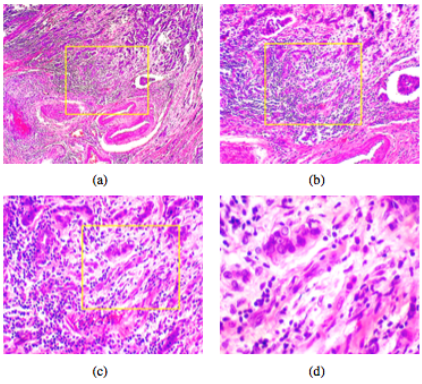
\includegraphics[width=0.8\textwidth]{logo.png}\par\vspace{1cm} % Imagen más grande
    {\scshape\Large Realizado por:\par}
    \vspace{1cm}
    {\Large \theauthor\par}
    \vfill
    {\large \thedate\par}
\end{titlepage}

% RESUMEN
\section*{Resumen}
Este proyecto se enmarca en la asignatura de Procesamiento de Imágenes Digitales (PID) y tiene como objetivo desarrollar un sistema que detecte el cáncer de mama mediante la identificación y comparación de células cancerígenas con células sanas. La metodología se basará en el uso de redes neuronales convolucionales (CNN) para analizar imágenes digitales de tejido mamario y extraer patrones característicos. Se realizan procesos de preprocesamiento y segmentación para aislar las áreas de interés, seguidos de la extracción de características específicas que permitan distinguir entre células malignas y benignas. Con este enfoque, se busca crear una herramienta de apoyo al diagnóstico clínico, que contribuya a una detección temprana y más precisa de la enfermedad.

\vspace{.5cm}

\textbf{Palabras clave:} cáncer de mama, redes neuronales convolucionales (CNN), células, benigno, maligno.

\newpage
% ÍNDICE
\tableofcontents

\newpage

% CONTENIDO
\section{Introducción}
El cáncer de mama es una de las principales causas de mortalidad en el mundo, habiendo sido la responsable de 670.000 muertes en 2022 siendo a su vez el tipo de cáncer más común en las mujeres según \cite{who_breast_cancer}. Esto provoca que durante los últimos años se haya estado realizando una labor social enorme referente a la concienciación sobre el cáncer de mama dando gran importancia a su pronta detección.\\

Gracias a los avances en Deep Learning \cite{shinde2018review}, se han desarrollado métodos innovadores para analizar imágenes histológicas y detectar el cáncer de mama. En este contexto, existen dos aproximaciones que se han estudiado en la literatura, como en el artículo textbf{“Classification of breast cancer based on histology images using convolutional neural networks}” \cite{bardou2018classification}, soportada por los 445 artículos en los que se realiza un estudio entre dos enfoques.\\

Este proyecto tiene como objetivo el desarrollo de una aplicación capaz de detectar cáncer de mama a partir de imágenes histológicas, utilizando dos enfoques complementarios. El primero se basa en una red neuronal convolucional (CNN) que realiza clasificación directamente a la imagen, y un segundo enfoque, basado en extracción de características seguida de la clasificación mediante el algoritmo K-Nearest Neighbors (KNN).\\

El enfoque basado en KNN está inspirado en el trabajo de \cite{bardou2018classification}, quienes proponen una combinación entre la codificación de características visuales utilizando técnicas como -bag of words y locality-constrained linear coding— y clasificadores tradicionales. En su estudio, se demostró que la extracción estructurada de características, combinada con métodos como KNN, puede lograr resultados competitivos en la clasificación de imágenes histológicas de cáncer de mama.\\

Por otro lado, el segundo enfoque se fundamenta en redes neuronales convolucionales, que han mostrado gran efectividad en la clasificación automática de imágenes biomédicas. Específicamente, el trabajo de \cite{minarno2021cnn} implementa un autoencoder basado en CNN para la recuperación de imágenes de cáncer de mama, permitiendo identificar imágenes similares dentro de grandes bases de datos. Esta capacidad de aprendizaje profundo permite al modelo extraer representaciones jerárquicas y semánticas directamente desde los datos crudos, sin necesidad de ingeniería manual de características.\\

Este último aprovecha la potencia de las Redes Neuronales Convolucionales (CNN), un tipo de red neuronal feedforward inspirada en la percepción visual \cite{hubel1962receptive}. Las CNN aplican filtros o “kernels” a lo largo de las imágenes para extraer automáticamente patrones y características como bordes, texturas y formas. Esta capacidad de aprender de forma automática elimina la necesidad de una extracción manual de atributos y, al reducir significativamente el número de conexiones en comparación con una red completamente conectada (FC), permite una convergencia más rápida y una actualización de pesos más eficiente durante el entrenamiento (véase Fig. \ref{fig:capas_convolucionales} Capas convolucionales).\\
\begin{figure}[!ht]
    \centering
    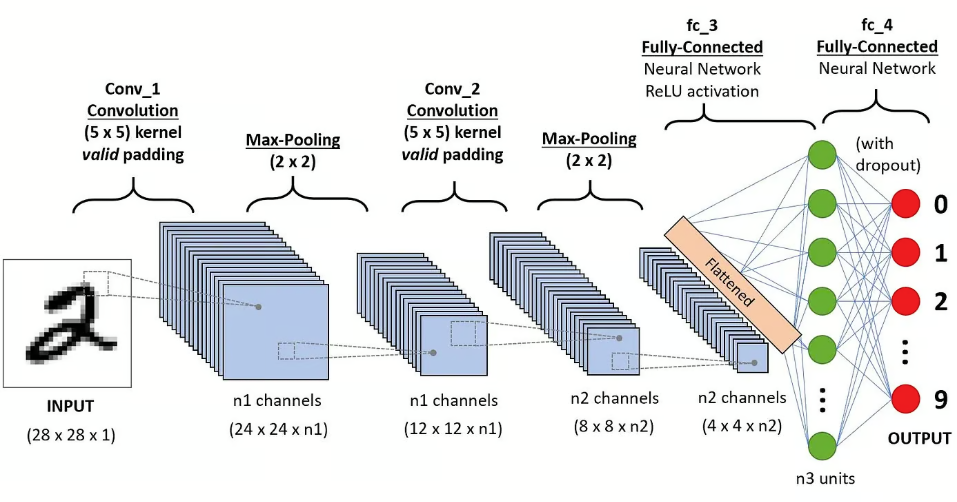
\includegraphics[width=0.8\textwidth]{CNN.png}
    \caption{Capas convolucionales \cite{datacamp_cnn}}
    \label{fig:capas_convolucionales}
\end{figure}\\

\newpage
Ambos enfoques son implementados y evaluados en este proyecto, comparando su rendimiento y su viabilidad para una futura aplicación en el diagnóstico asistido por computadora.\\

El objetivo de este proyecto es desarrollar un sistema que permita detectar el cáncer de mama a partir de imágenes histológicas, utilizando técnicas de aprendizaje automático y redes neuronales convolucionales. Se espera que este sistema contribuya a la mejora en la detección temprana del cáncer de mama, facilitando el trabajo de los profesionales médicos y aumentando la tasa de supervivencia de las pacientes.

El objetivo de nuestro trabajo es desarrollar una red convolucional capaz de detectar el cáncer de mama a partir de imágenes histológicas obtenidas de un dataset público [6] y comparar distintas aproximaciones para evaluar la eficacia en la detección temprana de esta enfermedad.

\section{Planteamiento del Teórico}
Contenido del marco teórico...

\subsection{Objetivos del Proyecto}
Este trabajo tiene como objetivo principal analizar y comparar diferentes metodologías de clasificación de imágenes médicas, con especial atención en la detección temprana del cáncer de mama. Para ello, se estudian tanto enfoques tradicionales de clasificación basados en extracción manual de características como enfoques modernos basados en aprendizaje profundo. Los objetivos específicos del proyecto son los siguientes:\\


\begin{enumerate}
    \item \textbf{Crear} una aplicacion que permita a los médicos detectar el cancer de mama solo dando la imagen.
    \item \textbf{Desarrollar} distintos modelos que permitan la clasificacion binaria de las imagenes.
    \item \textbf{Evaluar} el rendimiento de distintos modelos, tanto CNN en tareas de clasificación binaria como KNN.
    \item \textbf{Realizar experimentación para análisis} del  impacto de las técnicas de aumento de datos sobre el desempeño de los modelos.

\end{enumerate}

\section{Implementación}
Aquí van las conclusiones.

\section{Experimentación}
Aquí van las conclusiones.

\section{Manual de usuario}
Aquí van las conclusiones.

\section{Conclusiones}
Aquí van las conclusiones.

\section{Autoevaluación de cada miembro del equipo}
Aquí van las conclusiones.

\section{Tabla de tiempos}
Aquí van las conclusiones.

\addcontentsline{toc}{section}{Bibliografía} 
\printbibliography

\end{document}
